%%%%%%%%%%%%%%%%%%%%%%%%%%%%%%%%%%%%%%%%%
%
% (c) 2023 by Jennifer Laaser
%
% This work is licensed under the Creative Commons Attribution-NonCommercial-ShareAlike 4.0 International License. To view a copy of this license, visit http://creativecommons.org/licenses/by-nc-sa/4.0/ or send a letter to Creative Commons, PO Box 1866, Mountain View, CA 94042, USA.
%
% The current source for these materials is accessible on Github: https://github.com/jlaaser/pogil-polymers
%
%%%%%%%%%%%%%%%%%%%%%%%%%%%%%%%%%%%%%%%%%

\renewcommand{\figpath}{content/polymphys/extension-topics/block-copolymers/figs}
\renewcommand{\labelbase}{block-copolymers}

\begin{activity}[extension]{Block Copolymers}

\begin{instructornotes}

	This activity introduces students to key concepts related to self-assembly of block copolymers.
	
	After completing this activity, students will be able to:
			\begin{enumerate}
				\item \dots
			\end{enumerate}
	%This activity will prepare students for follow-up activities on phase diagrams for polymer solutions.
			
	\subsection*{Activity summary:}
	\begin{itemize}
		\item \textbf{Activity type:} Learning Cycle
		\item \textbf{Content goals:} See above %Ideal mixing, regular solution theory, and Flory-Huggins theory
		\item \textbf{Process goals:} %https://pogil.org/uploads/attachments/cj54b5yts006cklx4hh758htf-process-skills-official-pogil-list-2015-original.pdf
			\begin{itemize}
				\item \dots%Interpreting equations and figures
				\item %Applying equations to describe a model
				\item Written and oral communication of reasoning
			\end{itemize}
		\item \textbf{Duration:} TBD%approx. 75 minutes, including class discussion
			
		\item \textbf{Instructor preparation required:} none beyond knowledge of relevant content
		\item \textbf{Related textbook chapters:}
			\begin{itemize}
				\item \emph{Polymer Chemistry} (Hiemenz \& Lodge), 2nd ed.: sections \dots%7.1-7.3
				\item \emph{Introduction to Polymers} (Young \& Lovell), 3rd ed.: sections \dots%10.2.1 and 10.2.2
		\end{itemize}
	\end{itemize}

\end{instructornotes}

	%\textbf{Focus question:} Put a central question for the students to consider through this exercise here.

\begin{model}[Polymer Blends]
\label{\labelbase:mdl:polymerblends}

	Often, it is desirable to create blends of two chemically-different polymers, as depicted below:
	
	\vspace{6pt}
	\centerline{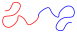
\includegraphics[width=0.9\textwidth]{\figpath/Model1_blend}}
	
	Following the same approach discussed for polymer solutions, it is possible to show that the free energy of mixing for this system is
	
	\begin{equation*}
		\frac{\Delta G}{kT} = \phi_A \phi_B \chi_{AB} + \frac{\phi_A}{N_A}\ln \phi_A + \frac{\phi_B}{N_B}\ln\phi_B
	\end{equation*}
	
	where $N_A$ and $N_B$ are the degrees of polymerization of the two polymers, $\phi_A$ and $\phi_B$ are their volume fractions, and $\chi_{AB}$ is their interaction parameter.

\end{model}

\vspace{0.05in}
\begin{ctqs}

	\question Which terms in the expression for $\Delta G$ given in the model represent the entropy of mixing?
	
		\begin{solution}[0.5in]
		\end{solution}
	
	\question When the polymer chains are long, $N_A$ and $N_B$ are large.  
	
		\begin{enumerate}
			\item What happens to the value of the entropic terms in this limit?
	
			\begin{solution}[1in]
			\end{solution}
	
			\item What happens to the value of $\Delta G$ in this limit, assuming that $\chi_{AB}>0$?
	
			\begin{solution}[1in]
			\end{solution}
		
		\end{enumerate}
	
	\question Based on your answers to the above questions, explain, in 2-3 complete sentences, why mixtures of chemically-different homopolymers tend to phase separate.
	
			\begin{solution}[1.5in]
			\end{solution}
	
	\question If the A and B polymers are linked together in a block copolymer, as shown below,
	
	\vspace{6pt}
	\centerline{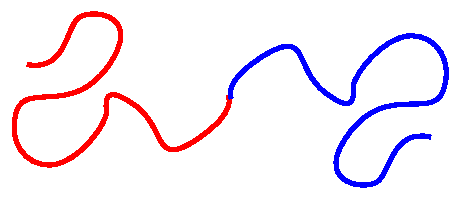
\includegraphics[width=0.2\textwidth]{\figpath/Model1_BCP}}
	
		will it be possible for them to phase separate in the same way?  If not, what do you expect them to do instead?  Explain your reasoning in 2-3 complete sentences.
	
			\begin{solution}[1.5in]
			\end{solution}
		
\end{ctqs}
	
	
\begin{model}[Block Copolymers]
\label{\labelbase:mdl:BCPs}

Block copolymers typically phase separate into ordered structures with dimensions on the order of 10s of nm.  The dimensions (and shapes) of these nanostructures depend on the sizes and compositions of the polymer chains.

As a simple example, we will consider the symmetric diblock copolymer depicted below, which phase separates into layered (``lamellar'') nanostructures:
	
	\vspace{6pt}
	\centerline{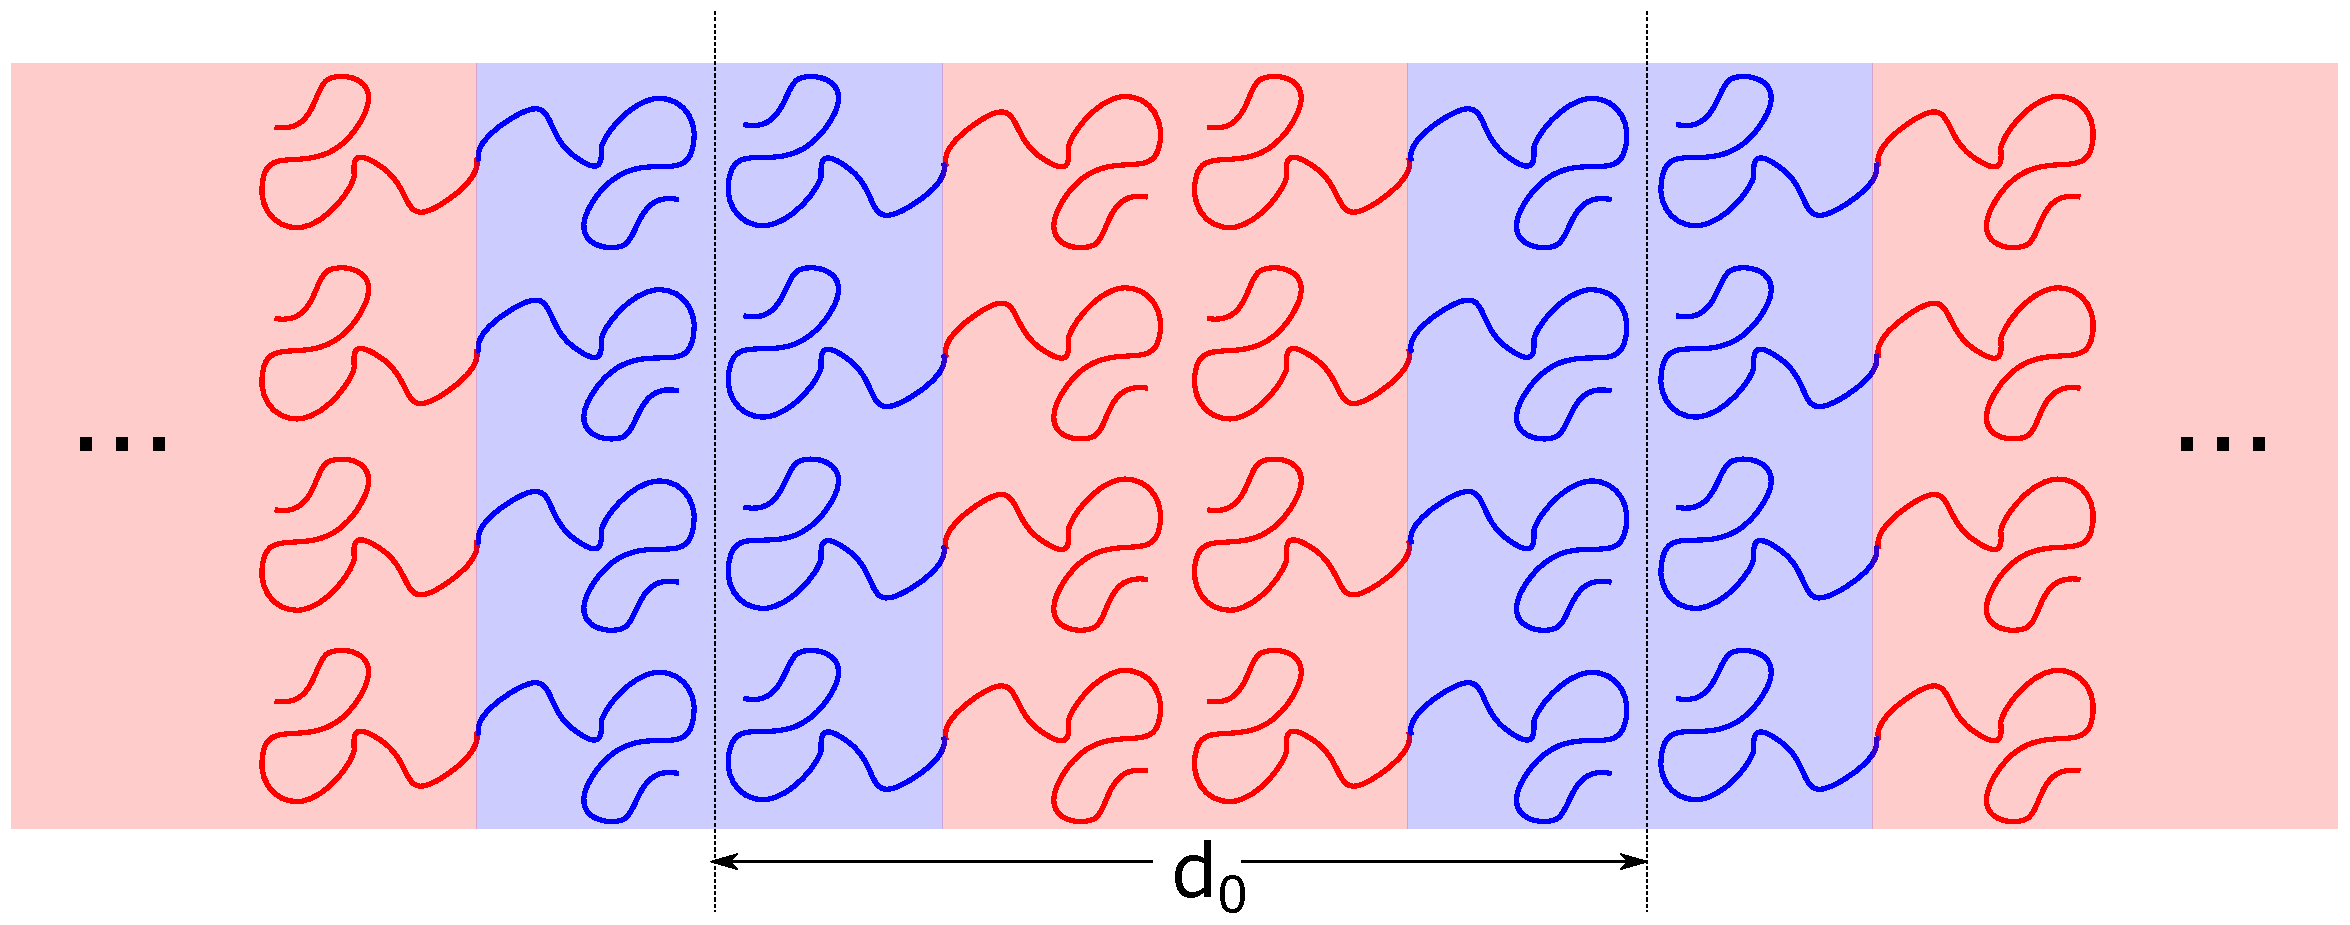
\includegraphics[width=0.6\textwidth]{\figpath/Model2_nanostructure}}

The characteristic spacing of the nanostructure (the length scale over which it repeats itself) is indicated by $d_0$.

\end{model}

\begin{ctqs}

	\question How is the characteristic spacing of the nanostructure related to the end-to-end distances of the individual chains?
	
		\begin{solution}[1in]
		\end{solution}
	
	\question Creating the nanostructure shown in Model \ref{\labelbase:mdl:BCPs} requires creating an interface between the A and B blocks, as shown below:
	
	\vspace{6pt}
	\centerline{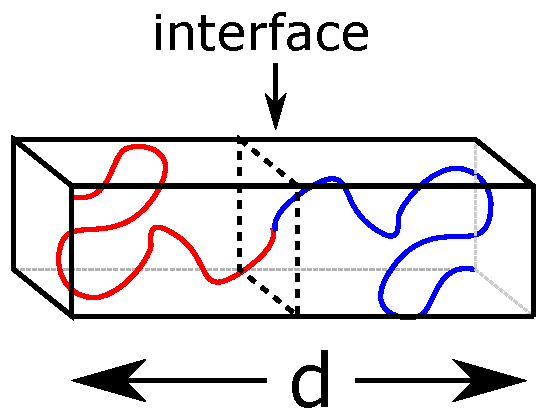
\includegraphics[width=0.3\textwidth]{\figpath/Model2_interface}}
	
		Assuming each chain has a total degree of polymerization of $N$ ($N = N_A + N_B$), and each monomer has volume $b^3$, determine...
	
		\begin{enumerate}
			\item ... the total volume of a single chain:
			
				\begin{solution}[0.5in]
					$V = Nb^3$
				\end{solution}
			
			\item ... the interfacial area, $\Sigma$, of a single chain, when its end-to-end distance is $d$?
			
				\begin{solution}[0.5in]
					$\Sigma = V/d = Nb^3/d$ 
				\end{solution}
			
		\end{enumerate}
	
	\question The enthalpy of the A/B interface is $\Delta H = \gamma_{AB} \Sigma$, where $\gamma_{AB} = \frac{k_B T}{b^2}\sqrt{\frac{\chi_{AB}}{6}}$.
	
		Does this enthalpy become more or less favorable as the domain spacing $d_0$ increases?  Explain your reasoning in 1-2 complete sentences.
	
		\begin{solution}[1.5in]
		\end{solution}
		
	\question The entropy change upon stretching a chain with $N$ monomers from end-to-end distance $h_0$ in its un-deformed conformation to end-to-end distance $h$ is $\Delta S = \frac{3k_B}{2Nb^2}(h_0^2 - h^2)$.
	
		Does this entropy become more or less favorable as the domain spacing $d_0$ increases?  Explain your reasoning in 1-2 complete sentences.
	
		\begin{solution}[1.5in]
		\end{solution}
		
	\question Write an expression for the Gibbs free energy for a symmetric diblock copolymer with $N$ monomers self-assembled into lamellae with principle domain spacing $d_0$.
	
		\begin{solution}[1in]
		\end{solution}
	
	\question What must be true about the value of $\Delta G$ when the system is in its ``best'' or ``preferred'' domain spacing?
	
		\begin{solution}[1in]
		\end{solution}
	
	\question Describe, in 2-3 complete sentences, how you would mathematically determine what this ``best'' or ``preferred'' domain spacing is for this system.
	
		\emph{Note: you do not need to actually do the math, but describe the process you would use!}
	
		\begin{solution}[1in]
		\end{solution}
		
\end{ctqs}

\begin{infobox}

	It is possible to show that the preferred domain spacing is
		\begin{equation*}
			d_0 = 1.03 b \chi_{AB}^{1/6} N^{2/3}
		\end{equation*}
		
	It is also possible to show that the minimum value of $\chi_{AB}$ required to form the ordered lamellar phase is approximately $10.5/N$; for smaller $\chi_{AB}$ values, the system will instead form a disordered melt.

\end{infobox}

\begin{ctqs}
		
	\question By what factor would doubling the molecular weight of the block copolymer change the characteristic domain spacing $d_0$?
	
		\begin{solution}[0.5in]
		\end{solution}
	
	\question Why do polymer physicists commonly say that the order-disorder transition occurs at $\chi N = 10.5$?
	
		\begin{solution}[0.5in]
		\end{solution}
	
\end{ctqs}


%\begin{exercises}
			
%		\exercise \dots
					
%\end{exercises}
	
\end{activity}